\documentclass[10pt,a4paper]{article}
\usepackage[utf8]{inputenc}
\usepackage{amsmath}
\usepackage{amsfonts}
\usepackage{amssymb}
\usepackage{graphicx}
\usepackage{caption}
\usepackage{subcaption}
\usepackage{float}
\usepackage{minted}
\usepackage[top=1.0in, bottom=1.0in, left=0.75in, right=0.75in]{geometry}
\author{Chittaranjan Srinivas Swaminathan and Anders Wikstrom}
\title{Scortec ER-I Manipulator Control using Arduino Due}
\begin{document}
\maketitle
\tableofcontents
\newpage
\section{Introduction}

\section{Description of task}
The Scortec ER-I is a 5-DOF manipulator from Eshed Robotec. The
control box is missing and a new controller is needed. For this
purpose, the Arduino Due board and a motor shield is used. \\

Figure \ref{fig:axes} shows a sketch of the manipulator and the axes.

\begin{figure}[h]
    \centering
    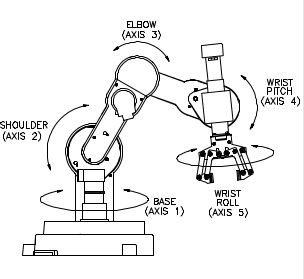
\includegraphics{axes.png}
    \caption{Scortec ER-I}
    \label{fig:axes}
\end{figure}

The task of creating a controller for the manipulator involves the
following steps:
\begin{enumerate}
\item Reverse engineer the motor and encoder connections and make a
  pinout diagram for the D50 connector on the manipulator.
\item Program the microcontroller to read the encoders.
\item Write control routines for position and velocity control.
\item Extend the control routines to more than one joint.
\end{enumerate}

The following sections describe each of these tasks and challenges
faced while executing them.

\section{Reverse Engineering}

In this task, we set out to map the pins on the D50 connector to the
individual motors and encoders. Once the pin-out diagram was in place
we could connect the Arduino and read the encoder pins. However, we
faced some problems while reading encoder outputs. The following
sections describe each of these tasks in detail. \\

\subsection{Pinout}
The primary task was to figure out the what each pin on the D50
connector meant. For this task we first took one motor and used the
multimeter to test for continuity. \\

\begin{figure}[h]
    \centering
    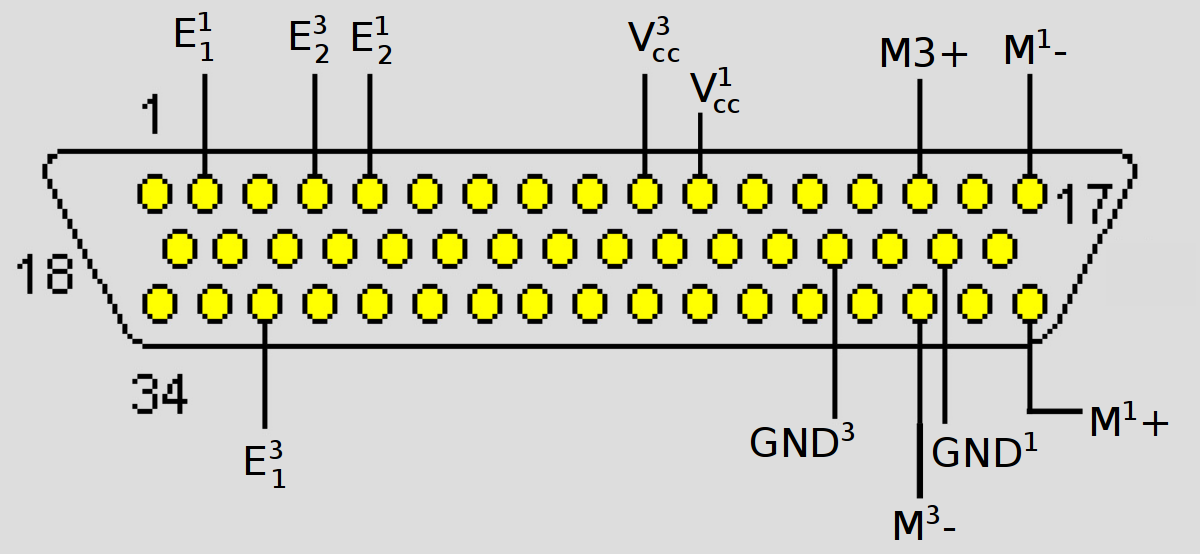
\includegraphics[scale=0.3]{dsub50.png}
    \caption{Pinout diagram for the D50 connector.}
    \label{fig:dsub}
\end{figure}

The figure \ref{fig:dsub} is the pinout diagram.\\
\( E^a_b \) refers to output of encoder \textit{b} on joint \textit{a}.\\
\( GND^a \) refers to ground for encoder board on joint \textit{a}.\\
\( V^a_{cc} \) refers to power supply for encoder board on joint
\textit{a}.\\ 
\( M^a+ \) refers to the positive pin on motor \textit{a}.\\

The motor has two pins (one positive and one negative) on the
connector. Each encoder board has a pair of encoders, thus enabling us
to read the incremental position of the joint as well as the direction
in which the joint is moving. The board has 6 pins but only 4 had
corresponding pins on the D50 connector. Also, it is important to
figure out what each of these pins meant.\\

To do this, we proceeded as follows:
\begin{enumerate}
\item The basic circuit for a Photodiode-LED pair is shown in figure
  \ref{fig:photodiodeLEDPair}. 
\item Detach the encoder board and use continuity test to figure out
  which components are connected.
\item Using the above two, figure out the circuit diagram of the
  board. This was found to be equivalent to figure
  \ref{fig:encoderCircuit}. 
\item Finally, relate each pin on the encoder board to the circuit.
\end{enumerate}

\begin{figure}[h]
    \centering
    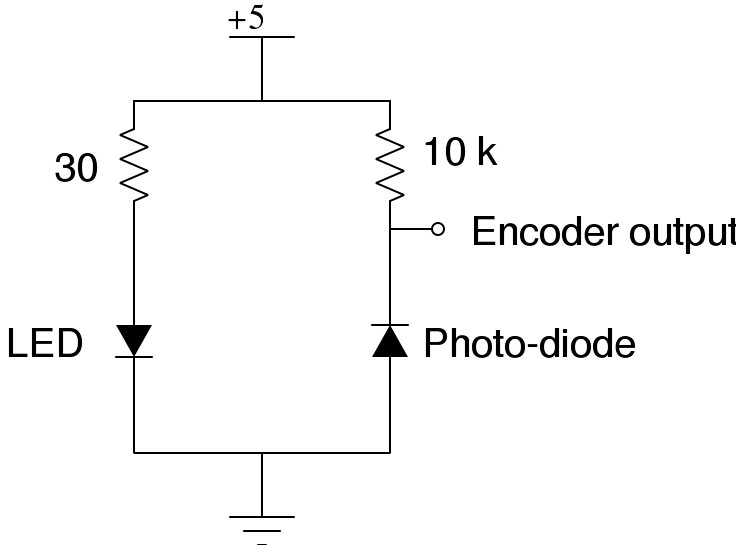
\includegraphics[scale=0.5]{SimpleEncoder.jpg}
    \caption{Basic circuit for Photodiode-LED pair.}
    \label{fig:photodiodeLEDPair}
\end{figure}

\begin{figure}[h]
    \centering
    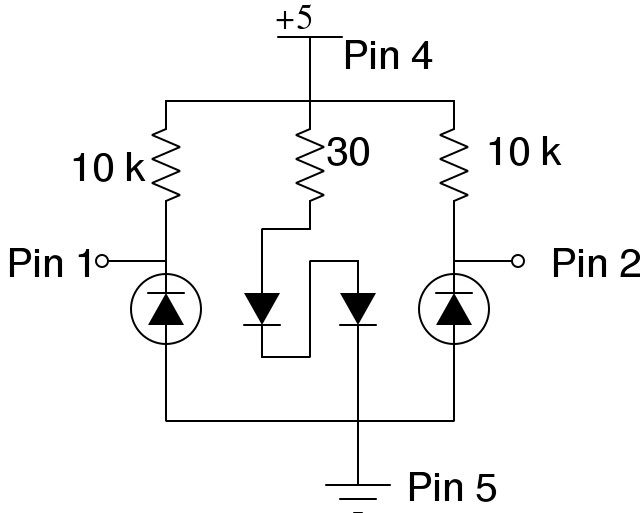
\includegraphics[scale=0.5]{EncoderCircuit.jpg}
    \caption{Equivalent Encoder circuitry with two Photodiode-LED
      pairs. The photodiode is circled.}
    \label{fig:encoderCircuit}
\end{figure}

\subsection{Debouncing}

\section{Control routines}

\subsection{Calibration}
\subsection{Velocity Control}
\subsection{Position Control}
\subsection{Overall organization of code}

\section{Evaluation of the system}

\subsection{Calibration}
\subsection{Accuracy and Precision for Joint 1}

\section{Future Work}

\end{document}